\documentclass{standalone}
\usepackage{tikz}
\usetikzlibrary{patterns, positioning}


\begin{document}
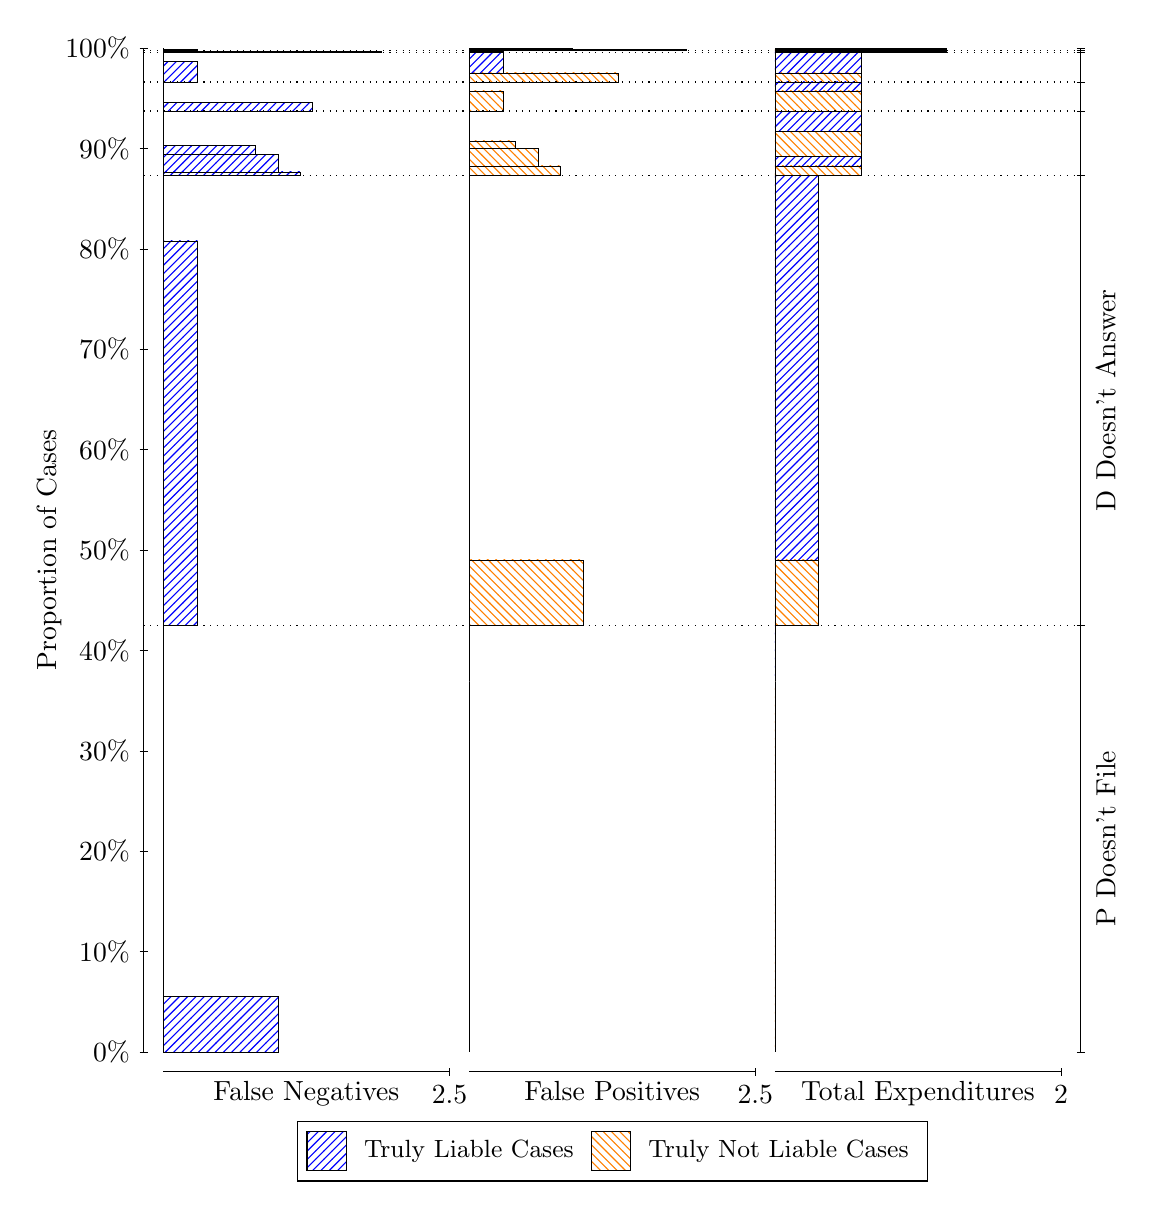
\begin{tikzpicture}
\draw[black, very thin] (1.5,1.75) -- (1.5,14.5);
\node[rotate=90, text=black, anchor=center] at (0.3, 8.125) {Proportion of Cases};
\draw[black, very thin] (1.45,1.75) -- (1.55,1.75);
\node[text=black, anchor=east] at (1.45, 1.75) {0\%};
\draw[black, very thin] (1.45,3.025) -- (1.55,3.025);
\node[text=black, anchor=east] at (1.45, 3.025) {10\%};
\draw[black, very thin] (1.45,4.3) -- (1.55,4.3);
\node[text=black, anchor=east] at (1.45, 4.3) {20\%};
\draw[black, very thin] (1.45,5.575) -- (1.55,5.575);
\node[text=black, anchor=east] at (1.45, 5.575) {30\%};
\draw[black, very thin] (1.45,6.85) -- (1.55,6.85);
\node[text=black, anchor=east] at (1.45, 6.85) {40\%};
\draw[black, very thin] (1.45,8.125) -- (1.55,8.125);
\node[text=black, anchor=east] at (1.45, 8.125) {50\%};
\draw[black, very thin] (1.45,9.4) -- (1.55,9.4);
\node[text=black, anchor=east] at (1.45, 9.4) {60\%};
\draw[black, very thin] (1.45,10.675) -- (1.55,10.675);
\node[text=black, anchor=east] at (1.45, 10.675) {70\%};
\draw[black, very thin] (1.45,11.95) -- (1.55,11.95);
\node[text=black, anchor=east] at (1.45, 11.95) {80\%};
\draw[black, very thin] (1.45,13.225) -- (1.55,13.225);
\node[text=black, anchor=east] at (1.45, 13.225) {90\%};
\draw[black, very thin] (1.45,14.5) -- (1.55,14.5);
\node[text=black, anchor=east] at (1.45, 14.5) {100\%};

\draw[black, very thin] (13.4,1.75) -- (13.4,14.5);
\draw[black, very thin] (13.35,1.75) -- (13.45,1.75);
\node[anchor=west] at (13.35, 1.75) {};
\draw[black, very thin] (13.35,7.1663) -- (13.45,7.1663);
\node[anchor=west] at (13.35, 7.1663) {};
\draw[black, very thin] (13.35,12.884) -- (13.45,12.884);
\node[anchor=west] at (13.35, 12.884) {};
\draw[black, very thin] (13.35,13.7) -- (13.45,13.7);
\node[anchor=west] at (13.35, 13.7) {};
\draw[black, very thin] (13.35,14.069) -- (13.45,14.069);
\node[anchor=west] at (13.35, 14.069) {};
\draw[black, very thin] (13.35,14.443) -- (13.45,14.443);
\node[anchor=west] at (13.35, 14.443) {};
\draw[black, very thin] (13.35,14.471) -- (13.45,14.471);
\node[anchor=west] at (13.35, 14.471) {};
\draw[black, very thin] (13.35,14.5) -- (13.45,14.5);
\node[anchor=west] at (13.35, 14.5) {};

\draw[black, very thin, pattern color=blue, pattern=north east lines] (1.75,1.75) rectangle (3.2033,2.4609);
\draw[black, very thin, pattern color=orange, pattern=north west lines] (1.75,2.4609) rectangle (1.75,7.1663);
\draw[black, very thin, pattern color=blue, pattern=north east lines] (1.75,7.1663) rectangle (2.186,12.051);
\draw[black, very thin, pattern color=orange, pattern=north west lines] (1.75,12.051) rectangle (1.75,12.884);
\draw[black, very thin, pattern color=blue, pattern=north east lines] (1.75,12.884) rectangle (3.494,12.926);
\draw[black, very thin, pattern color=blue, pattern=north east lines] (1.75,12.926) rectangle (3.2033,13.146);
\draw[black, very thin, pattern color=blue, pattern=north east lines] (1.75,13.146) rectangle (2.9127,13.263);
\draw[black, very thin, pattern color=orange, pattern=north west lines] (1.75,13.263) rectangle (1.75,13.7);
\draw[black, very thin, pattern color=blue, pattern=north east lines] (1.75,13.7) rectangle (3.6393,13.812);
\draw[black, very thin, pattern color=orange, pattern=north west lines] (1.75,13.812) rectangle (1.75,14.069);
\draw[black, very thin, pattern color=blue, pattern=north east lines] (1.75,14.069) rectangle (2.186,14.328);
\draw[black, very thin, pattern color=orange, pattern=north west lines] (1.75,14.328) rectangle (1.75,14.443);
\draw[black, very thin, pattern color=blue, pattern=north east lines] (1.75,14.443) rectangle (4.5113,14.456);
\draw[black, very thin, pattern color=orange, pattern=north west lines] (1.75,14.456) rectangle (1.75,14.471);
\draw[black, very thin, pattern color=blue, pattern=north east lines] (1.75,14.471) rectangle (2.186,14.486);
\draw[black, very thin, pattern color=orange, pattern=north west lines] (1.75,14.486) rectangle (1.75,14.5);
\draw[black, very thin, pattern color=orange, pattern=north west lines] (5.6333,1.75) rectangle (5.6333,6.4554);
\draw[black, very thin, pattern color=blue, pattern=north east lines] (5.6333,6.4554) rectangle (5.6333,7.1663);
\draw[black, very thin, pattern color=orange, pattern=north west lines] (5.6333,7.1663) rectangle (7.0867,7.9996);
\draw[black, very thin, pattern color=blue, pattern=north east lines] (5.6333,7.9996) rectangle (5.6333,12.884);
\draw[black, very thin, pattern color=orange, pattern=north west lines] (5.6333,12.884) rectangle (6.796,13.002);
\draw[black, very thin, pattern color=orange, pattern=north west lines] (5.6333,13.002) rectangle (6.5053,13.226);
\draw[black, very thin, pattern color=orange, pattern=north west lines] (5.6333,13.226) rectangle (6.2147,13.321);
\draw[black, very thin, pattern color=blue, pattern=north east lines] (5.6333,13.321) rectangle (5.6333,13.7);
\draw[black, very thin, pattern color=orange, pattern=north west lines] (5.6333,13.7) rectangle (6.0693,13.956);
\draw[black, very thin, pattern color=blue, pattern=north east lines] (5.6333,13.956) rectangle (5.6333,14.069);
\draw[black, very thin, pattern color=orange, pattern=north west lines] (5.6333,14.069) rectangle (7.5227,14.183);
\draw[black, very thin, pattern color=blue, pattern=north east lines] (5.6333,14.183) rectangle (6.0693,14.443);
\draw[black, very thin, pattern color=orange, pattern=north west lines] (5.6333,14.443) rectangle (6.0693,14.458);
\draw[black, very thin, pattern color=blue, pattern=north east lines] (5.6333,14.458) rectangle (5.6333,14.471);
\draw[black, very thin, pattern color=orange, pattern=north west lines] (5.6333,14.471) rectangle (8.3947,14.485);
\draw[black, very thin, pattern color=blue, pattern=north east lines] (5.6333,14.485) rectangle (6.9413,14.5);
\draw[black, very thin, pattern color=orange, pattern=north west lines] (9.5167,1.75) rectangle (9.5167,6.4554);
\draw[black, very thin, pattern color=blue, pattern=north east lines] (9.5167,6.4554) rectangle (9.5167,7.1663);
\draw[black, very thin, pattern color=orange, pattern=north west lines] (9.5167,7.1663) rectangle (10.062,7.9996);
\draw[black, very thin, pattern color=blue, pattern=north east lines] (9.5167,7.9996) rectangle (10.062,12.884);
\draw[black, very thin, pattern color=orange, pattern=north west lines] (9.5167,12.884) rectangle (10.607,13.002);
\draw[black, very thin, pattern color=blue, pattern=north east lines] (9.5167,13.002) rectangle (10.607,13.119);
\draw[black, very thin, pattern color=orange, pattern=north west lines] (9.5167,13.119) rectangle (10.607,13.438);
\draw[black, very thin, pattern color=blue, pattern=north east lines] (9.5167,13.438) rectangle (10.607,13.7);
\draw[black, very thin, pattern color=orange, pattern=north west lines] (9.5167,13.7) rectangle (10.607,13.956);
\draw[black, very thin, pattern color=blue, pattern=north east lines] (9.5167,13.956) rectangle (10.607,14.069);
\draw[black, very thin, pattern color=orange, pattern=north west lines] (9.5167,14.069) rectangle (10.607,14.183);
\draw[black, very thin, pattern color=blue, pattern=north east lines] (9.5167,14.183) rectangle (10.607,14.443);
\draw[black, very thin, pattern color=orange, pattern=north west lines] (9.5167,14.443) rectangle (11.697,14.458);
\draw[black, very thin, pattern color=blue, pattern=north east lines] (9.5167,14.458) rectangle (11.697,14.471);
\draw[black, very thin, pattern color=orange, pattern=north west lines] (9.5167,14.471) rectangle (11.697,14.485);
\draw[black, very thin, pattern color=blue, pattern=north east lines] (9.5167,14.485) rectangle (11.697,14.5);
\draw[black, dotted] (1.5,7.1663) -- (13.4,7.1663);
\draw[black, dotted] (1.5,12.884) -- (13.4,12.884);
\draw[black, dotted] (1.5,13.7) -- (13.4,13.7);
\draw[black, dotted] (1.5,14.069) -- (13.4,14.069);
\draw[black, dotted] (1.5,14.443) -- (13.4,14.443);
\draw[black, dotted] (1.5,14.471) -- (13.4,14.471);
\draw[black, very thin] (1.75,1.5) -- (5.3833,1.5);
\node[text=black, anchor=north] at (3.5667, 1.5) {False Negatives};
\draw[black, very thin] (5.3833,1.45) -- (5.3833,1.55);
\node[text=black, anchor=north] at (5.3833, 1.45) {2.5};

\draw[black, very thin] (5.6333,1.5) -- (9.2667,1.5);
\node[text=black, anchor=north] at (7.45, 1.5) {False Positives};
\draw[black, very thin] (9.2667,1.45) -- (9.2667,1.55);
\node[text=black, anchor=north] at (9.2667, 1.45) {2.5};

\draw[black, very thin] (9.5167,1.5) -- (13.15,1.5);
\node[text=black, anchor=north] at (11.333, 1.5) {Total Expenditures};
\draw[black, very thin] (13.15,1.45) -- (13.15,1.55);
\node[text=black, anchor=north] at (13.15, 1.45) {2};

\node[text=black, centered, rotate=90] at (13.72, 4.4582) {P Doesn't File};
\node[text=black, centered, rotate=90] at (13.72, 10.025) {D Doesn't Answer};






\draw (7.449999999999999,1.5) node[draw=none] (baseCoordinate) {};
\begin{scope}[align=center]
        \matrix[scale=0.5, draw=black, below=0.5cm of baseCoordinate, nodes={draw}, column sep=0.1cm]{
            \node[rectangle, draw, minimum width=0.5cm, minimum height=0.5cm, pattern color=blue, pattern=north east lines] {}; &
            \node[draw=none, font=\small, text=black] (B) {Truly Liable Cases}; &
            \node[rectangle, draw, minimum width=0.5cm, minimum height=0.5cm, pattern color=orange, pattern=north west lines] {}; &
            \node[draw=none, font=\small, text=black] (B) {Truly Not Liable Cases}; \\
            };
\end{scope}

\end{tikzpicture}
\end{document}